%%%%%%%%%%%%%%%%%%%%%%%%%%%%%%%%%%%%%%%%%%%%%%%%%%%%%%%%%%%%%%%%%%%%%%%%%%%%%
%%%%%%                                                                  %%%%% 
%%%%%%          Maqueta de memòria TFC/PFC de l'EETAC                   %%%%% 
%%%%%%                                                                  %%%%% 
%%%%%%%%%%%%%%%%%%%%%%%%%%%%%%%%%%%%%%%%%%%%%%%%%%%%%%%%%%%%%%%%%%%%%%%%%%%%%
%%%%%%%%%%%%%%%%%%%%%%%%%%%%%%%%%%%%%%%%%%%%%%%%%%%%%%%%%%%%%%%%%%%%%%%%%%%%%
%%                                                                         %%
%%          Autor: Xavier Prats i Menéndez (xavier.prats@upc.edu)          %% 
%%                  Technical University of Catalonia (UPC)                %%
%%                                                                         %%
%%%%%%%%%%%%%%%%%%%%%%%%%%%%%%%%%%%%%%%%%%%%%%%%%%%%%%%%%%%%%%%%%%%%%%%%%%%%%
%%      This work is licensed under the Creative Commons  Attribution-     %%
%%   -Noncommercial-Share Alike 3.0 Spain License. To view a copy of this  %% 
%%    license, visit http://creativecommons.org/licenses/by-nc-sa/3.0/es/  %%
%%    or send a letter to Creative Commons, 171 Second Street, Suite 300,  %%
%%                  San Francisco,California, 94105, USA.                  %%
%%%%%%%%%%%%%%%%%%%%%%%%%%%%%%%%%%%%%%%%%%%%%%%%%%%%%%%%%%%%%%%%%%%%%%%%%%%%%
%% Versió 2.1 - Juliol 2012                                                %%
%%%%%%%%%%%%%%%%%%%%%%%%%%%%%%%%%%%%%%%%%%%%%%%%%%%%%%%%%%%%%%%%%%%%%%%%%%%%%

%%% NOTA: els seguents packages son necessaris per utilitzar la
%%%       plantilla seguent:
%%%       ifthen,calc,helvet,pslatex,fancyhdr,nextpage,subfigure,tocloft,graphicx,url

%%% NOTA: Es possible que algunes distribuicions Linux o Windows.
%%%       no portin aquests paquets instal·lats per defecte.
%%%       En aquest cas els haureu d'instal·lar manualment.


%%%%%%%%%%%%%%%%%%%%%%%%%%%%%%%%%%%%%%%%%%%%%%%%%%%%%%%%%%%%%%%%%%%%%%%%%%%%%
% 1- INICIALITZACIÓ
%%%%%%%%%%%%%%%%%%%%%%%%%%%%%%%%%%%%%%%%%%%%%%%%%%%%%%%%%%%%%%%%%%%%%%%%%%%%%

\documentclass[english,final]{setup/eetac_tfc_pfc}
%% * OPCIONS A CONFIGURAR al \documentclass
%%    - Estat del document: final o draft
%%      NOTA: Draft no inserta les figures i marca només l'espai que
%%      ocupen. També s'indica quan el text sobrepassa els marges.
%%      Draft és molt útil per compilar ràpid el document si no és important
%%      en aquell moment visualitzar les figures.
%%    - Idioma PRINCIPAL del document: catalan, spanish, english, french...

\usepackage[english]{babel}
%%  * INCLOURE TOTS ELS IDIOMES QUE S'USARAN EN EL DOCUMENT
%%    NOTA: per canviar d'idioma al mig del document usar:
%%          \selectlanguage{nom_idioma}
%%%%%%%%%%%%%%%%%%%%%%%%%%%%%%%%%%%%%%%%%%%%%%%%%%%%%%%%%%%%%%%%%%%%%%%%%%%%%

%%%%%%%%%%%%%%%%%%%%%%%%%%%%%%%%%%%%%%%%%%%%%%%%%%%%%%%%%%%%%%%%%%%%%%%%%%%%%
% 2- CÀRREGA DE PAQUETS ADICIONALS (OPCIONALS)
%%%%%%%%%%%%%%%%%%%%%%%%%%%%%%%%%%%%%%%%%%%%%%%%%%%%%%%%%%%%%%%%%%%%%%%%%%%%%

%%% NOTA: Es possible que algunes distribuicions Linux o Windows.
%%%       no portin aquests paquets instal·lats per defecte.
%%%       En aquest cas els haureu d'instal·lar manualment.

%% El paquet inputenc és extramadament útil. 
%% Permet escriure els accents directament amb l'editor de texte
%% sense haver de fer coses com per exemple: introducci\'o
%% Heu d'especificar la codificació de caracters que utilitzeu pel
%% vostre fitxer (en aquest exemple utf8)
\usepackage[utf8]{inputenc}

%% Símbols matemàtics de la American Mathematical Society
\usepackage{amssymb, amsmath, amsfonts}  

%% El paquet array proporciona eines molt útils a l'hora de fer 
%% equacions amb matrius
\usepackage{array}             

%% Paquet que permet fer taules fusionant cel·les de files consecutives
\usepackage{multirow}          

%% Paquet molt útil en cas de tenir taules molt llargues que 
%   ocupin vàries pàgines
\usepackage{longtable}          

%% Permet canviar els colors del document
\usepackage{color,colortbl}

%% Paquet molt útil que permet activar links en el PDF final.
\usepackage[
  	% CUSTOM PDF 
  	pdfauthor={Fernando Román García},
  	pdftitle={Master thesis - Fernando Román García},
	pdfsubject={An enhanced SleuthKit GUI for digital forensics},
	pdfkeywords={digital, forensics, sleuth, kit, GUI},
	%
  	pdfcreator={EETAC-UPC},
	pdfproducer={LaTeX, dvipdf},
	pdfdisplaydoctitle=true,
  	plainpages=false,
	linktocpage=true,
	colorlinks=true,
  	linkcolor=blue,
	citecolor=blue,
	urlcolor=blue,
	hyperfootnotes=false,
  	pagebackref=true,
	pdfpagelabels=true,
	pdfpagemode=UseOutlines,
]{hyperref} 

%% NOTA IMPORTANT!:
%% Per tal que hyperef funcioni correctament amb els capitols o seccions no
%% numerats (\chapter*{}), com per exemple introducció, conclusions i
%% bibliografia cal posar les dues comandes seguents ABANS del \chapter*{} en
%% questió
%\cleardoublepage \phantomsection

%% Permet trencar links URL. 
%% Atenció! afegir aquest paquet DESPRES del hyperref!!
\usepackage{breakurl} 

%% Permet arranjar matricialment multiples figures
%% NOTA: afegir aquest paquet DESPRES del hyperref!!
%%       Si no es desitja utilitzar aquest paquet, comentar la linia seguent
%%       i anar TAMBE al fitxer de classe (eetac_tfc_pfc.cls) per substituir: 
%%       \RequirePackage[subfigure]{tocloft}  per  \RequirePackage{tocloft}
\usepackage{subfigmat}

% Custom packages
\usepackage{xparse}
\usepackage{listings}
\usepackage{rotating}
\usepackage{pdflscape}
\usepackage{wrapfig}
\usepackage{etoolbox}

%%%%%%%%%%%%%%%%%%%%%%%%%%%%%%%%%%%%%%%%%%%%%%%%%%%%%%%%%%%%%%%%%%%%%%%%%%%%%
% 3- DOCUMENT
%%%%%%%%%%%%%%%%%%%%%%%%%%%%%%%%%%%%%%%%%%%%%%%%%%%%%%%%%%%%%%%%%%%%%%%%%%%%%

%%% Configuració de les dades i variables boleanes rellevants del document:
%%%%%%%%%%%%%%%%%%%%%%%%%%%%%%%%%%%%%%%%%%%%%%%%%%%%%%%%%%%%%%%%%%%%%%%%%%%%%
%%%%%%                                                                  %%%%% 
%%%%%%       Fitxer de dades per la memoria TFC/PFC de l'EETAC          %%%%% 
%%%%%%                                                                  %%%%% 
%%%%%%%%%%%%%%%%%%%%%%%%%%%%%%%%%%%%%%%%%%%%%%%%%%%%%%%%%%%%%%%%%%%%%%%%%%%%%
%%%%%%%%%%%%%%%%%%%%%%%%%%%%%%%%%%%%%%%%%%%%%%%%%%%%%%%%%%%%%%%%%%%%%%%%%%%%%
%%                                                                         %%
%%          Autor: Xavier Prats i Menendez (xavier.prats@upc.edu)          %% 
%%                  Technical University of Catalonia (UPC)                %%
%%                                                                         %%
%%%%%%%%%%%%%%%%%%%%%%%%%%%%%%%%%%%%%%%%%%%%%%%%%%%%%%%%%%%%%%%%%%%%%%%%%%%%%
%%      This work is licensed under the Creative Commons  Attribution-     %%
%%   -Noncommercial-Share Alike 3.0 Spain License. To view a copy of this  %% 
%%    license, visit http://creativecommons.org/licenses/by-nc-sa/3.0/es/  %%
%%    or send a letter to Creative Commons, 171 Second Street, Suite 300,  %%
%%                  San Francisco,California, 94105, USA.                  %%
%%%%%%%%%%%%%%%%%%%%%%%%%%%%%%%%%%%%%%%%%%%%%%%%%%%%%%%%%%%%%%%%%%%%%%%%%%%%%
%% Versio 2.1 - Juliol 2012                                                %%
%%%%%%%%%%%%%%%%%%%%%%%%%%%%%%%%%%%%%%%%%%%%%%%%%%%%%%%%%%%%%%%%%%%%%%%%%%%%%

%%%%%%%%%%%%%%%%%%%%%%%%%%%%%%%%%%%%%%%%%%%%%%%%%%%%%%%%%%%%%%%%%%%%%%%%%%%%%%%
%%  VARIABLES A CONFIGURAR                                                  %%%
%%%%%%%%%%%%%%%%%%%%%%%%%%%%%%%%%%%%%%%%%%%%%%%%%%%%%%%%%%%%%%%%%%%%%%%%%%%%%%%

%% - Projecte o Treball de Fi de Carrera?
%%      PFC = true   -> Projecte de Fi de Carrera
%%      PFC = false  -> Treball  de Fi de Carrera
\setboolean{PFC}{false}

%% - Escollir la titulació
%\titulacio{Enginyeria Tècnica Aeronàutica, especialitat Aeronavegació}
%\titulacio{Enginyeria T\`ecnica de Telecomunicaci\'o, especialitat Sistemes de Telecomunicaci\'o}
%\titulacio{Enginyeria T\`ecnica de Telecomunicaci\'o, especialitat Telem\`atica}
%\titulacio{Enginyeria de Telecomunicaci\'o (segon cicle)}
% Modificació respecte a la versió 2.1 - Iván Padilla Montero - Juliol 2014
\titulacio{Grau en Enginyeria d'Aeronavegaci\'o}
%\titulacio{Grau en Enginyeria d'Aeroports}
%\titulacio{Grau en Enginyeria Telemàtica}
%\titulacio{Grau en Enginyeria de Sistemes de Telecomunicació}


%% - Configurar els idiomes del document
%% Si l'idioma PRINCIPAL del document es l'angles, posar aquesta variable a true
\setboolean{Leng}{false}

%% Escollir entre catala i castella (idioma principial, o nomes pel resum en cas que l'idioma principal sigui anglès)
%%  catala = true   -> idioma principal (o només resum) en Català
%%  catala = false  -> idioma principal (o només resum) en Castella
\setboolean{Lcat}{true}

%% Titol del document en l'idioma principal del document 
\titol{Això és el Títol del Document}

%% Titol del document en anglès (Per l'apartat overview)
\titolE{This is the Document's title}

%% Titol del document en catala/castella (Per l'apartat resum)
\titolC{Això és el Títol del Document}


%% - Nombre d'autors del TFC/PFC?
%%      UNautor = true   Un sol autor
%%      UNautor = false  Més d'un autor
\setboolean{UNautor}{false}

%% - Nom del(s) Autor(s) del document
%% NOTA: En cas de mes d'un autor cal posar la comana \and entre els
%%        noms dels autors
\autor{Nom1 Cognoms1 \and Nom2 Cognoms2 \and  Nom3 Cognoms3}

%% - Nombre de directors del TFC/PFC. Tipicament 1 o 2
%%      UNdirector = true   Un sol director
%%      UNdirector = false  Dos directors
\setboolean{UNdirector}{false}

%% - Nom del Director del TFC/PFC
\director{Nom1 Cognoms1}

%% - Nom del segon director en cas de tenir-lo:
\segonDirector{Nom2 Cognoms2}


%% - Es vol incloure una dedicatoria?
%%      dedicatoria = true   -> S'afegeix una pagina amb \textDedicatoria
%%      dedicatoria = true   -> No s'afegeix dedicatoria
%% NOTA: no confondre dedicatòria amb agraïments. Una dedicatoria sol ser
%%       un missatge curt d'una o dues frases màxim a la persona, o persones
%%       a les quals es dedica el treball. 
%%       Els agraïments poden ser extensos i l'autor pot agraïr a diverses
%%       persones coses diferents en funció de l'ajuda rebuda, per exemple. 
%%       Si es volen incloure agraïments, fer-ho al fitxer de la 
%%       memòria creant una secció nova amb  \chapter*{Agraïments}
\setboolean{dedicatoria}{true}
\textDedicatoria{Escriure aqui \\ la dedicatòria}

%% - Es vol incloure una pagina d'index de figures?
\setboolean{paginaLOF}{true}  % List of Figures

%% - Es vol incloure una pagina d'index de taules?
\setboolean{paginaLOT}{true}  % List of Tables 

%% - El projecte ha estat supervisat per alguna persona externa? 
%%   (NOMES en cas de practiques en empresa)
%%      supervisor = true    -> Hi ha un supervisor
%%      supervisor = false   -> No hi ha un supervisor
\setboolean{supervisor}{true}

%% NOMES en el cas de practiques en empresa (supervisor=true) s'han de 
%% configurar les variables seguents: 

%% Supervisor del TFC/PFC 
\supervisor{Nom del Supervisor}

%% - Es vol incloure el logotip de l'empresa?
%%   En el cas que el TFC/PFC s'hagi fet en règim d'intercanvi amb una
%%   empresa, es pot afegir el seu logotip a la cantonada superior
%%   dreta de la portada. En aquest cas:
%%   - posar logo=true
%%   - posar el path de la imatge i l'alçada del logo a \mylogo
\setboolean{logo}{false}
\mylogo{./setup/EETAC-positiu-negre}{1.5cm}
  

%%% Configuració de MACROS o ENTORNS (opcionals) definides per l'usuari:
%%%%%%%%%%%%%%%%%%%%%%%%%%%%%%%%%%%%%%%%%%%%%%%%%%%%%%%%%%%%%%%%%%%%%%%%%%%%%
%%%%%%                                                                  %%%%% 
%%%%%%    Fitxer de macros d'usuari per la memoria TFC/PFC de l'EETAC   %%%%% 
%%%%%%                                                                  %%%%% 
%%%%%%%%%%%%%%%%%%%%%%%%%%%%%%%%%%%%%%%%%%%%%%%%%%%%%%%%%%%%%%%%%%%%%%%%%%%%%
%%%%%%%%%%%%%%%%%%%%%%%%%%%%%%%%%%%%%%%%%%%%%%%%%%%%%%%%%%%%%%%%%%%%%%%%%%%%%
%%                                                                         %%
%%         Author: Xavier Prats i Menendez (xavier.prats@upc.edu)          %% 
%%                  Technical University of Catalonia (UPC)                %%
%%                                                                         %%
%%%%%%%%%%%%%%%%%%%%%%%%%%%%%%%%%%%%%%%%%%%%%%%%%%%%%%%%%%%%%%%%%%%%%%%%%%%%%
%%      This work is licensed under the Creative Commons  Attribution-     %%
%%   -Noncommercial-Share Alike 3.0 Spain License. To view a copy of this  %% 
%%    license, visit http://creativecommons.org/licenses/by-nc-sa/3.0/es/  %%
%%    or send a letter to Creative Commons, 171 Second Street, Suite 300,  %%
%%                  San Francisco,California, 94105, USA.                  %%
%%%%%%%%%%%%%%%%%%%%%%%%%%%%%%%%%%%%%%%%%%%%%%%%%%%%%%%%%%%%%%%%%%%%%%%%%%%%%
%% Versio 1.5 - Juliol 2010                                                %%
%%%%%%%%%%%%%%%%%%%%%%%%%%%%%%%%%%%%%%%%%%%%%%%%%%%%%%%%%%%%%%%%%%%%%%%%%%%%%


%%% Xevi's macros for vectors and matrices:

%\newcommand{\ve}[1]{\mbox{\boldmath$#1$}}          
\newcommand{\ve}[1]{\vec{#1}}  
\newcommand{\ma}[1]{\mbox{\boldmath$\mathcal{#1}$}}

%%% Xevi's macros for brackets:
\newcommand{\lp}{\left(}
\newcommand{\lc}{\left[}
\newcommand{\lcl}{\left\{}
\newcommand{\rp}{\right)}
\newcommand{\rc}{\right]}
\newcommand{\rcl}{\right\}}

%%% Xevi's new environment for HIPOTESIS
\newcounter{num_hyp}
\newenvironment{hyp}[2]{
        \refstepcounter{num_hyp}
        \vspace*{2.5ex}
        {\noindent \bf\sffamily HYPOTHESIS #1 : #2} \\
        \sl
}
        {\vspace{1ex}
}

\newcommand{\SUMhyp}[2]{
 {\sffamily HYPOTHESIS #1 : #2} 
}

\newcommand{\icon}[2]{%
	$\null\mathsurround=0pt$%
	\includegraphics[height=\dimexpr\fontdimen22\textfont2+1ex\relax]{#1}
	\textbf{#2.}\space}

\def\CC{{C\nolinebreak[4]\hspace{-.05em}\raisebox{.3ex}{\small\bf ++}\space}}

\newcommand{\approxtext}[1][]{%
	\ensuremath{\stackrel{\text{#1}}{\approx}}
}  

%%% Configuració manual de les regles d'hyphenation:
%%%%%%%%%%%%%%%%%%%%%%%%%%%%%%%%%%%%%%%%%%%%%%%%%%%%%%%%%%%%%%%%%%%%%%%%%%%%%
%%%%%%                                                                  %%%%% 
%%%%%%    Fitxer de hyphenation per la memoria TFC/PFC de l'EETAC       %%%%% 
%%%%%%                                                                  %%%%% 
%%%%%%%%%%%%%%%%%%%%%%%%%%%%%%%%%%%%%%%%%%%%%%%%%%%%%%%%%%%%%%%%%%%%%%%%%%%%%
%%%%%%%%%%%%%%%%%%%%%%%%%%%%%%%%%%%%%%%%%%%%%%%%%%%%%%%%%%%%%%%%%%%%%%%%%%%%%
%%                                                                         %%
%%         Author: Xavier Prats i Menendez (xavier.prats@upc.edu)          %% 
%%                  Technical University of Catalonia (UPC)                %%
%%                                                                         %%
%%%%%%%%%%%%%%%%%%%%%%%%%%%%%%%%%%%%%%%%%%%%%%%%%%%%%%%%%%%%%%%%%%%%%%%%%%%%%
%%      This work is licensed under the Creative Commons  Attribution-     %%
%%   -Noncommercial-Share Alike 3.0 Spain License. To view a copy of this  %% 
%%    license, visit http://creativecommons.org/licenses/by-nc-sa/3.0/es/  %%
%%    or send a letter to Creative Commons, 171 Second Street, Suite 300,  %%
%%                  San Francisco,California, 94105, USA.                  %%
%%%%%%%%%%%%%%%%%%%%%%%%%%%%%%%%%%%%%%%%%%%%%%%%%%%%%%%%%%%%%%%%%%%%%%%%%%%%%
%% Versio 1.5 - Juliol 2010                                                %%
%%%%%%%%%%%%%%%%%%%%%%%%%%%%%%%%%%%%%%%%%%%%%%%%%%%%%%%%%%%%%%%%%%%%%%%%%%%%%

\hyphenation{Cas-tell-de-fels}
\hyphenation{EETAC}
  

%%% Configurations of programming languages highlights 
%%% MOVE THIS TO MACRO FILE?? %%%

% Colors %%%%%%%%%%%%%%%%%%%%%%%%%%%%%%%%%%%%%%%%%%%%%%%%%%%%%%%%%%%%%%%%%%%%%%%

\definecolor{dkgreen}{rgb}{0,0.6,0}
\definecolor{gray}{rgb}{0.5,0.5,0.5}
\definecolor{mauve}{rgb}{0.58,0,0.82}
\definecolor{deepblue}{rgb}{0,0,0.5}
\definecolor{deepred}{rgb}{0.6,0,0}
\definecolor{deepgreen}{rgb}{0,0.5,0}

\definecolor{pictonblue}{RGB}{62, 193, 233}
\definecolor{turquoiseblue}{rgb}{0.388,0.831,0.960}
\definecolor{saffron}{rgb}{0.372,0.211,0.988}
\definecolor{rawsienna}{rgb}{0.819,0.576,0.255}

\definecolor{brightedred}{RGB}{161,0,0}
\definecolor{gigas}{RGB}{72, 62, 170}


% Custom macros %%%%%%%%%%%%%%%%%%%%%%%%%%%%%%%%%%%%%%%%%%%%%%%%%%%%%%%%%%%%%%%%

\newcommand{\lstcustomdefaults}{
	\setkeys{lst}{
		basicstyle=\footnotesize\ttfamily,
		aboveskip=3mm,
		belowskip=3mm,
		showstringspaces=false,
		columns=flexible,
		numbers=left,
		numberstyle=\footnotesize,
		breaklines=true,
		breakatwhitespace=true,
		tabsize=3,
	}
}
\newcommand{\newproglanguage}[2]{
	\expandafter\newcommand\csname #1style\endcsname[1][]{
		#2
		\lstcustomdefaults
		\setkeys{lst}{##1}
	}
	
	\lstnewenvironment{#1}[1][]
	{
		\expandafter\csname #1style\endcsname
		\lstset{##1}
	}
	{}
	
	\expandafter\DeclareDocumentCommand\csname #1external\endcsname
	{ O{} m }
	{
		\expandafter\csname #1style\endcsname
		\lstinputlisting[##1]{##2}
	}
	
	\expandafter\newcommand\csname #1inline\endcsname
	[1]{{\expandafter\csname #1style\endcsname\lstinline!##1!}}
}

%% Code figure
\newenvironment{codefigure}[2]{
	\begin{figure}[htb]
		\begin{quote}
			\def\codeFigCaption{#1}
			\def\codeFigLabel{#2}
}
{
			\caption{\codeFigCaption}
			\label{\codeFigLabel}
		\end{quote}
	\end{figure}
}

%% Bash code
\newenvironment{bashcode}{
	\begin{center}\itshape\bfseries
}
{
	\end{center}
}


% Style highlighting %%%%%%%%%%%%%%%%%%%%%%%%%%%%%%%%%%%%%%%%%%%%%%%%%%%%%%%%%%%

%% Java
\newproglanguage{java}{
	\lstset{
		language=Java,
		basicstyle={\small\ttfamily},
		numberstyle=\tiny\color{gray},
		keywordstyle=\color{blue},
		commentstyle=\color{dkgreen},
		stringstyle=\color{mauve},
	}
}

%% Python
\newproglanguage{python}{
	\lstset{
		language=Python,
		otherkeywords={self},             	% Add keywords here
		keywordstyle=\color{deepblue},
		emph={
			__init__,
			TestApp,
			App,
			Button
		},          				    	% Custom highlighting
		emphstyle=\color{deepred},    		% Custom highlighting style
		stringstyle=\color{deepgreen},
	}
}

%% C++
\newproglanguage{cpp}{
	\lstset{
		language=C++,
		% Language settings
		commentstyle=\color{dkgreen}\ttfamily,
		identifierstyle=\color{black},
		stringstyle=\color{red}\ttfamily,
		% Syntax keywords
		classoffset=0,
		keywordstyle=\color{blue},
		% Classes
		classoffset=1,
		keywordstyle=\color{turquoiseblue}\bfseries,
	}
}


%% JavaScript
\lstdefinelanguage{JavaScript}{
	% Language settings
	sensitive=true,
	% Keywords
	classoffset=0,
	keywords={typeof, new, true, false, catch, function, return,
		null, catch, switch, var, if, in, while, do, else, case,
		break, const, let, class, export, boolean, throw, implements,
		default, import, this, extends},
	% Classes
	classoffset=1,
	keywords={Math},
	% Comments
	comment=[l]{//},
	morecomment=[s]{/*}{*/},
	% Strings
	morestring=[b]',
	morestring=[b]",
}
\newproglanguage{js}{
	\lstset{
		language=JavaScript,
		% General theme
		commentstyle=\color{dkgreen}\ttfamily,
		identifierstyle=\color{black},
		stringstyle=\color{red}\ttfamily,
		% Syntax keywords
		classoffset=0,
		keywordstyle=\color{gigas}\bfseries,
		% Classes
		classoffset=1,
		keywordstyle=\color{turquoiseblue}\bfseries,
	}
}


%% JSX
\lstdefinelanguage{JSX}{
	% Language settings
	alsoletter={<, >, \/},
	sensitive=true,
	% Keywords
	classoffset=0,
	keywords={typeof, new, true, false, catch, function, return,
		null, catch, switch, var, if, in, while, do, else, case,
		break, const, let, class, export, boolean, throw, implements,
		default, import, this, extends},
	% HTML
	classoffset=2,
	keywords={<div>, <\/div>, />},
	% Comments
	comment=[l]{//},
	morecomment=[s]{/*}{*/},
	% Strings
	morestring=[b]',
	morestring=[b]",
}
\newproglanguage{jsx}{
	\lstset{
		language=JSX,
		% General theme
		commentstyle=\color{dkgreen}\ttfamily,
		identifierstyle=\color{black},
		stringstyle=\color{red}\ttfamily,
		% Syntax keywords
		classoffset=0,
		keywordstyle=\color{gigas}\bfseries,
		% Classes
		classoffset=1,
		keywordstyle=\color{turquoiseblue}\bfseries,
		% HTML
		classoffset=2,
		keywordstyle=\color{black}\bfseries,
	}
}

%% Haxe
\lstdefinelanguage{Haxe}{
	% General theme
	sensitive=true,
	% Syntax keywords
	classoffset=0,
	keywords={class, static, public, function, var},
	% Classes
	classoffset=1,
	keywordstyle={String, Void},
	% Comments
	comment=[l]{//},
	morecomment=[s]{/*}{*/},
	% Strings
	morestring=[b]',
	morestring=[b]"
}
\newproglanguage{haxe}{
	\lstset{
		language=Haxe,
		% General theme
		commentstyle=\color{dkgreen}\ttfamily,
		stringstyle=\color{red}\ttfamily,
		identifierstyle=\color{black},
		% Syntax keywords
		classoffset=0,
		keywordstyle=\color{blue}\bfseries,
		% Classes
		classoffset=1,
		keywordstyle=\color{turquoiseblue}\bfseries,
	}
}


%% Sass
\lstdefinelanguage{Sass}{
	alsoletter={-, :, \#, .},
	sensitive=false,
	% CSS properties
	classoffset=0,
	keywords={background-color:, color:, display:, flex:},
	% SCSS @ methods
	classoffset=1,
	keywords={@include, @mixin},
	% User defined variables and classes
	classoffset=2,
	% Comments
	comment=[l]{//},
	morecomment=[s]{/*}{*/},
	% Strings
	morestring=[b]',
	morestring=[b]"
}
\newproglanguage{sass}{
	\lstset{
		language=Sass,
		% General theme
		commentstyle=\color{dkgreen}\ttfamily,
		stringstyle=\color{red}\ttfamily,
		identifierstyle={\color{gigas}\small\ttfamily},
		% CSS properties
		classoffset=0,
		keywordstyle=\color{brightedred}\bfseries,
		% SCSS @ methods
		classoffset=1,
		keywordstyle=\color{black}\bfseries,
		% User defined variables and classes
		classoffset=2,
		keywordstyle=\color{pictonblue},
	}
}



\begin{document}

%% Seleccionar l'idioma principal del document:
\selectlanguage{english}

\beforepreface  

%% RESUM i OVERVIEW
%%%%%%%%%%%%%%%%%%%%%%%%%%%%%%%%%%%%%%%%%%%%%%%%%%%%%%%%%%%%%%%%%%%%%%%%%%%%%
% NOTA: les longituds passades com a parametres d'entrada  s'han d'ajustar
% manualment fins que el requadre del resum/overview ocupi tota la pàgina. 

%%% Resum en català (o castellà)
%\begin{resum}{10cm} Aquest document conté les pautes del format de presentació
%del treball o projecte de %final de carrera. En tot cas, cal tenir en compte
%el que estableix la ``Normativa del %treball de fi de carrera (TFC) i del
%projecte de fi de carrera (PFC)'' aprovada per la %Comissió Permanent de
%l'EETAC, especialment l'apartat ``Requeriments del treball''.  \end{resum}

%%% Resum en anglès
\begin{overview}{11cm} This document contains guidelines for writing your
TFC/PFC. However, you should also take into consideration the standards
established in the document Normativa del treball de fi de carrera (TFC) i del
projecte de fi de carrera (PFC), paying special attention to the section
Requeriments del treball, as this document has been approved by the EETAC
Standing Committee \end{overview}


%NOTA: En cas d'utilitzar l'espanyol com a idioma principal del document, el
%latex anomena les taules com a 'Cuadros'. Si es desitja canviar aquesta
%nomenclatura i utilitzar la paraula 'Tabla' descomentar les línies següents:
%\def\listtablename{Índice de tablas} \def\tablename{Tabla}%



% Amb aqueta comanda indiquem que ja s'han inclòs tots els apartats del prefaci
% del projecte o podem començar a incloure els capitols de la memòria
\afterpreface


%%%%%%%%%%%%%%%%%%%%%%%%%%%%%%%%%%%%%%%%%%%%%%%%%%%%%%%%%%%%%%%%%%%%%%%%%%
%%%%%% INCLOURE A PARTIR D'AQUÍ TOTS ELS CAPÍTOLS DE LA MEMORIA   %%%%%%%%
%%%%%%%%%%%%%%%%%%%%%%%%%%%%%%%%%%%%%%%%%%%%%%%%%%%%%%%%%%%%%%%%%%%%%%%%%%

% NOTA: recordar que la introducció i les conclusions són capítols NO
% enumerats, per tant s'ha d'usar \chapter*

% NOTA: és aconsellable incloure els capítols de la memòria en fitxers separats
% utlitzant la comanda \input  Per exemple: \input{capitol1}  que farà que
% s'inclogui el fitxer capitol1.tex

% NOTA: Si es vol incloure agraïments i/o glosari, fer-ho utilitzant
% \chapter*{} i incloure'ls abans la introducció

\cleardoublepage
\phantomsection
\chapter*{Introduction}
L'objectiu d'aquest document és donar unes pautes per a la presentació dels projectes o treballs de fi de carrera fets amb l'entorn \LaTeX. Aquest document és, en si mateix, un exemple de la presentació d'aquest treball en aquest format i pot fer-se servir (es recomana) com a plantilla per editar a sobre la pròpia memòria del TFC/PFC.

Els fitxers \LaTeX \ necessaris han estat escrits per Xavier Prats i Menéndez, professor de la EETAC, per tal d'oferir una alternativa als estudiants a l'hora de redactar les seves memòries de TFC/PFC. Si detecteu qualsevol error o teniu algun suggeriment per millorar aquesta plantilla i el corresponent fitxer de classe, podeu adreçar-vos a directament a \emph{xavier.prats@upc.edu}. Cal dir, que només s'atendran consultes o problemes sobre els fitxers d'estil i la plantilla proporcionada i en cap cas es donarà suport sobre la utilització i la sintaxi de les comanes \LaTeX. Existeix, tant a Internet com a les biblioteques de la UPC, una  bibliografia abundant i útil en aquest sentit. 

Al primer capítol es poden trobar totes les instruccions relatives a la forma de presentació, és a dir, el tipus de lletra, el paper, els marges, els encapçalaments, la numeració, i totes aquelles qüestions que afecten el treball o projecte en conjunt.

Al segon capítol es marquen les instruccions que afecten cada part del treball, com poden ser: la portada, el resum, l'índex i el cos del document.

% \chapter{Digital forensics}

% TODO
De wikipedia! Redatar otra vez

Digital forensics (sometimes known as digital forensic science) is a branch of
forensic science encompassing the recovery and investigation of material found
in digital devices, often in relation to computer crime.[1][2] The term digital
forensics was originally used is a synonym for computer forensics but has
expanded to cover investigation of all devices capable of storing digital
data.[1] With roots in the personal computing revolution of the late 1970s and
early 1980s, the discipline evolved in a haphazard manner during the 1990s, and
it was not until the early 21st century that national policies emerged.

The goal of computer forensics is to explain the current state of a digital
artifact; such as a computer system, storage medium or electronic document.[38]
The discipline usually covers computers, embedded systems (digital devices with
rudimentary computing power and onboard memory) and static memory (such as USB
pen drives).

Computer forensics can deal with a broad range of information; from logs (such
as internet history) through to the actual files on the drive.

In 2007 prosecutors used a spreadsheet recovered from the computer of Joseph E.
Duncan III to show premeditation and secure the death penalty.[3] Sharon
Lopatka's killer was identified in 2006 after email messages from him detailing
torture and death fantasies were found on her computer.

\section{Phases}

% TODO
SOME TEXT HERE



\section{Tools}

% TODO
What's a digital forensic tool??

\subsection{The Sleuth Kit and Autopsy}

\subsection{The Coroner's Toolkit}


\chapter{Cross-platform development}

At the beginning of computers, each hardware manufacturer had to decide how
access to its hardware functionalities. Since there were no standards for some
cases, the first inter-compatibility problems started to appear because
programs were not able to run on different computers.

To reduce these problems drivers were created. A driver is a piece of code that 
maps logic functions (for instance, turn on a led) to hardware operations 
(short circuit some part of the electronics). Programs call this logic functions
so for them it's not important how to turn on the led, is the driver who 
specifies how to do it. Then, for software, the only important part is how these
functions are called.

Logic functions are provided to programs by the Operative Systems (OS) so the 
problem now is that not all OS use the same functions names.

\section{Technological soup}

Nowadays lots of technologies has been created with the goal of writing just
one code to run in as many platforms possible. We want to achieve this
in order to reduce the development cost, but this results in a performance
reduction.

The most intuitive solution may be to use cross-platform frameworks to perform
the functions that have problems with interoperability. These frameworks have 
conditionals that execute a logic function or another depending on which 
operative system is the one that is compiling this library.

But the common way to achieve this goal is with scripting programming
languages. These are human readable text and are interpreted by a program
called interpreter during the execution time. One step further is to compile
them into pseudo-machine code that is easy to understand for the interpreter.
This second group of is known as virtual machine programming languages. This
have the advantage that programs are faster, but developers lose some time
compiling the code each time they want to test something. Both technologies can
run over all the platforms that its interpreter is supported.

Another kind of solutions are transcompilers or source-to-source compilers. They
translate from one programming language to many others. This translation could
be done in a scripting language (there interoperability is provided) or can make
a specific translation to a compiled language depending on the OS.

\subsection{Java}

This well-known programming language is one of the most used to build
cross-platform applications due to its maturity. Java is a general-purpose,
concurrent, classbased, object-oriented language and it's designed to be easy
to learn in order to let many programmers to have fluency in the language
\cite{java-8-specs}.

Classic compiled languages, such as, C and C++, directly compile into machine
code, which is directly interpreted by the hardware. As opposed to C and C++,
Java can be considered a virtual machine programming language.

\begin{codefigure}{Java hello world}{F:java-hello-world}
	\javaexternal{source/HelloWorldApp.java}
\end{codefigure}

Figure \ref{F:java-hello-world} is an example of Java program that prints the
test “Hello World!” into the terminal.

\subsection{Qt}

A complete cross-platform software framework with ready-made UI elements, C++ 
libraries, and a complete integrated development environment with tools for 
everything you need to develop software for any project \cite{qt-web}.

\begin{codefigure}{Qt hello world}{F:qt-hello-world}
	\cppexternal{source/qt_hello_world.cpp}
\end{codefigure}

\subsection{Python}

This is an example of a scripting programming language. The main design rule
was to be very easy to read.

It's also a considered an object-oriented language suitable for many purposes.
It has a clear, intuitive syntax, powerful high-level data structures, and a
flexible dynamic type system \cite{An93pythonfor}.

Python is often used to create terminal programs or web services because GUI
are not supported by default but there are many frameworks that can be used,
for instance, \textbf{Kivy}.

\begin{codefigure}{Kivy hello world}{F:kivy-hello-world}
	\pythonexternal{source/kivy_hello_world.py}
\end{codefigure}

\subsection{JavaScript}

JavaScript is also a well know scripting programming language. It's used
alongside with HTML and CSS as core technologies to make any webpages. But due
to its flexibility is used on many other fields as game programming or desktop
applications.

It has many interpreters but all of them has to fulfill ECMAScript 
specification. V8 is an example of JavaScript engine used in Google Chrome and
Node.js. This latest is to build desktop applications in JavaScript.

Developing trends of last years to create cross-platform applications were to 
develop a web application because all platforms have browsers. For this reason,
web technologies grow a lot but the problem is that the user experience of a
web page will never be as good as using a desktop application.

\subsubsection{Electron}

Electron is a Node.js framework that lets you build cross-platform desktop apps
with JavaScript, HTML, and CSS \cite{electron-web}. Since web technologies, due
to web applications, has grown, now are able to race with other desktop
technologies. The idea of Electron is to take profit of the fact that Node.js
and Chrome use the same JavaScript engine to let Node instantiate browser
windows that also run Node.js.

So using Electron, developers are able to create cross-platform desktop 
applications using the same technologies that the ones used to create a web
page.

\subsubsection{NW.js}

NW.js, previously known as node-webkit, works on the contrary of Electron. It's
a Chrome web browser where you can call all the node modules \cite{nwjs-web}.
So the main difference is the entry point of the application. In Electron, the
start point of your program execution is Node.js while on NW.js the entry point
is an HTML file.

\subsection{Haxe}

Finally, Haxe is a high-level open source programming language that can be 
transcompiled many other languages. It has an ECMAScript-oriented syntax but 
with the peculiarity that can be typed \cite{what-is-haxe}. 

\begin{table}[htb]
\begin{center}
\begin{tabular}{|l|l|l|}
\hline
{\bf Name }		& {\bf Output Type} & {\bf Main usages}  \\ \hline \hline
JavaScript		& Sourcecode		& Browser, Desktop, Mobile, Server \\ \hline
Neko			& Bytecode			& Desktop, Server   \\ \hline
PHP				& Sourcecode		& Server   \\ \hline
Python			& Sourcecode		& Desktop, Server   \\ \hline
C++				& Sourcecode		& Desktop, Mobile, Server   \\ \hline
ActionScript 3	& Sourcecode		& Browser, Desktop, Mobile   \\ \hline
Flash			& Bytecode			& Browser, Desktop, Mobile   \\ \hline
Java			& Sourcecode		& Desktop, Server   \\ \hline
C\#				& Sourcecode		& Desktop, Mobile, Server   \\ \hline
\end{tabular}
\caption{Haxe use cases \cite{what-is-haxe}}
\label{T:haxe-use-cases}
\end{center}
\end{table}

Table \ref{T:haxe-use-cases} shows up many languages in which Haxe can be
compiled. Then lets see a bit of Haxe syntax.

\begin{codefigure}{Haxe hello world}{F:haxe-hello-world}
	\haxeexternal[
		classoffset=1,
		morekeywords={Main}
	]{source/Main.hx}
\end{codefigure}

As we can see in Figure \ref{F:haxe-hello-world}, Haxe can be typed defining 
variables that way: \haxeinline{var text: String}. Then, this code can be
compiled for example to Python other languages using the terminal command:

\begin{bashcode}
	haxe -main Main.hx -python \textless\text{outfile.py}\textgreater
\end{bashcode}

\section{Electron}

The technology that fits better with the project specifications is Electron. 
There are several projects like this one that are developed using this 
framework. Even it is not as mature as other ones it had a bit impact in the
developers community.

% TODO: PUT SOME EXAMPLES?? 
% Visual Studio Code, Atom, Slack, Github Desktop

Furthermore, the development of web applications has been evolved very fast with
the objective to have complex programs with a very good scalability and without
putting so much effort.

Now lets see how it works a little more in detail. Complete code of following 
examples can be seen on Appendix BLABLA

% TODO: CREATE APPENDIX

\subsection{Main process}

Since JavaScript is single threaded, to work in parallel Electron have several
processes. The initial one is called main process. It in charge of create all
browser windows, communicate them, to build application menus and control
context events.

\begin{codefigure}{Electron app events}{F:electron-app-events}
	\jsexternal{source/electron-app.js}
\end{codefigure}

Code of Figure \ref{F:electron-app-events} is an example of the most common
handled events. The most important is the \textit{"ready"} event, which is in
charge to create the main window of the application.

\subsection{Browser window}

Once event \textit{"ready"} is called, browser windows can be created. Each
window have its own process and are called renderer processes. The way to
create windows is shown on Figure \ref{F:electron-create-window}.

\begin{codefigure}{Electron window creation}{F:electron-create-window}
	\jsexternal[
		classoffset=1,
		morekeywords={BrowserWindow},
	]{source/electron-create-window.js}
\end{codefigure}

Browser windows can be created using several parameters to define its initial
behavior, for instance: width, height, position, etc. Also, they can load files 
using several protocols. In Electron, the most common way is to use local files
to reduce the load time and let the application work without Internet 
connection. And finally applications also have events, for example: 
\textit{"closed"}, \textit{"ready-to-show"}, \textit{"move"}\dots

\subsection{Menu and context menu}

% TODO: DE MOMENTO NADA

\subsection{Interprocess communication}

Finally, to be able to communicate the main process and renderer processes, 
Electron provides an interprocess communication system (IPC). It can be both
ways, main to renderer and renderer to main.

To communicate two renderer processes, a bridge must be created inside the 
main process.

\section{Web technologies}

To improve project's scalability and maintainability several web technologies
are used.

\subsection{Typescript}

Typescript is typed superset of JavaScript that compiles to plain JavaScript
created by Microsoft \cite{typescript-web}. It has two main advantages:

\begin{description}
	\item[Typed language]
	Since Typescript is a typed language and it has a compilation process, any
	mismatch of parameters in a function call can be detected. This is useful
	to check if something is not well programmed before test the application.
	
	Also, Integrated Development Environments (IDEs) can help developers before
	type mismatches happens because now this information is provided.
	
	\item[Compiles to plain Javascript]
	There are many web browsers and not all of them are not providing the same
	JavaScript functionalities. To use TypeScript allows developer to not take
	care of it because is the compiler who chooses the proper JavaScript code.

\end{description}

Many JavaScript libraries also provide its TypeScript typings. Using this 
information, the compiler can detect if the library is properly used.

Each time TypeScript is compiled, a tool called TsLint can be used to
check if some programming style guides are followed. They help to keep the code
easy-to-read because some rules are used, for instance: the use of lower camel 
case for variables and upper camel case for classes.

\subsection{Sass}

Like Typescript is a code transcompiler, but it translates from sass to css. It
is designed to improve CSS functionalities.

\begin{codefigure}{Sass example}{F:sass-example}
	\sassexternal[
		classoffset=2,
		morekeywords={\$app_green, flex-row}
	]{source/example.scss}
\end{codefigure}

Figure \ref{F:sass-example} helps to see all the advantages that Sass provides.
The main of them are:

\begin{description}
	\item[Nesting CSS selectors]
	Improves code scalability. 
	
	\item[Variables]
	Helps to define palettes, sizes, etc.
	
	\item[Mixins]
	They are similar to functions. Is very useful to define common behaviors.
	
\end{description}

% TODO: Explicar que se ha estructurado scss por componentes visuales??

\subsection{Gulp}

Gulp is a toolkit for automating painful or time-consuming tasks in your
development workflow, so you can stop messing around and build something
\cite{gulp-web}.

This project has several routine tasks, such as launch electron, compile
Typescript and Sass each time a file change happens, etc. For this reason, 
several gulp tasks to help development.

% TODO: Poner un ejemplo de una tarea de gulp configurada??
\chapter{Software architecture}

% TODO



\section{React + Redux}

\subsection{React}

\subsection{Redux}

\subsection{Integration}

\section{Other packages}

\subsection{Redux Observables}

\subsection{React Redux Form}

\subsection{React Tables}

\section{TSK-JS}


\chapter{Digital forensics analysis}
\label{S:df-analysis}

The Sleuth Kit (TSK) is an open source cross-platform collection of terminal
applications and a C library that allows investigators to analyze disk images
and recover files from them \cite{tsk-web}. It is divided in file system and
volume tools. 

The first group allows investigators to examine the file system of a suspect
computer in a non-intrusive way. Main file system tools are shown on Table
\ref{T:tsk-fs-tools}.

\begin{table}[htb]
\begin{center}
\begin{tabular}{|l|l|l|}
\hline
{\bf Command }	& {\bf Description }  \\ \hline \hline
fsstat & Shows file system details and statistics \\ \hline \hline
fls	& Lists allocated and deleted file names in a directory \\ \hline
ffind & Finds allocated and unallocated file names \\ \hline \hline
icat & Extracts the data units of a file \\ \hline
\end{tabular}
\caption{Main file system tools from TSK \cite{tsk-tools-wiki}}
\label{T:tsk-fs-tools}
\end{center}
\end{table}

Volume tools are the ones that brings off the layout of disks and another media.
They are needed to identify where partitions are located to be able to proceed
with a file system analysis. Table \ref{T:tsk-v-tools} lists main volume tools.

\begin{table}[htb]
\begin{center}
\begin{tabular}{|l|l|l|}
\hline
{\bf Command }	& {\bf Description }  \\ \hline \hline
mmls & Displays the layout of a disk \\ \hline \hline
mmstat & Display details about a volume system \\ \hline
\end{tabular}
\caption{Main volume tools from TSK \cite{tsk-tools-wiki}}
\label{T:tsk-v-tools}
\end{center}
\end{table}

In order to explain how The Sleuth Kit works easily, an example will be used.
In that specific case, an investigator will extract the timeline for an image
and will look for a file called \textit{letter.txt} to print its content.

\section{The Sleuth Kit analysis}
\label{S:tsk-analysis}

To start the TSK analysis, the command \textit{mmls} is used to output the 
information of all partitions. If volume type is not specified, TSK will
autodetect it. The output will look like Listing \ref{L:tsk-mmls-output}.
This example has tree volumes:

\begin{description}
	\item [Primary Table (\#0)]
	It contains the primary table. 
	
	\item [Unallocated]
	Unallocated space.

	\item [Win95 FAT32 (0x0C)]
	This partition has an offset of 56 sectors and it contains a file system formatted with FAT32.
	
\end{description}

\begin{terminal}[caption=TSK mmls output example, label=L:tsk-mmls-output]
	%
	\terminalcmd[mmls hdd-001.dd]
	%
	DOS Partition Table
	Offset Sector: 0
	Units are in 512-byte sectors
	
	Slot         Start        End          Length       Description
	00:  Meta    0000000000   0000000000   0000000001   Primary Table (#0)
	01:  -----   0000000000   0000000055   0000000056   Unallocated
	02:  00:00   0000000056   0007925759   0007925704   Win95 FAT32 (0x0C)
	%\terminalcmd%
\end{terminal}

To perform a deeper analysis, file system tools must be used. In that case,
those will need the offset of 56 sectors to be specified. The  first tool,
\textit{fsstat}, will display some file system characteristics, for instance,
root inode, sector size and the file system layout.

Also, the registers inside the disk can be listed in a non-intrusive way using 
\textit{fls}. In this specific example (Listing \ref{L:fls-output-example}),
the file system contains four folders. One of them,  
\textit{\_NTITL\textasciitilde1} is deleted. Also, some virtual registers are
displayed (\$MBR, \$FAT1, \$FAT2, \$OrphanFiles). If it is necessary to go
through the file system tree, a directory inode can be specified to list
registers inside it or analyze whole disk recursively.

\begin{terminal}[caption=TSK fls output example,label=L:fls-output-example]
%
\terminalcmd[fls -o 56 hdd-001.dd]
%
d/d 4:	.Trash-1000
d/d * 5:	_NTITL~1
d/d 7:	Personal
d/d 9:	Imagenes
v/v 126563459:	$MBR
v/v 126563460:	$FAT1
v/v 126563461:	$FAT2
d/d 126563462:	$OrphanFiles
%\terminalcmd%
\end{terminal}

Several times, it is necessary to export the whole file system in order to obtain
processed information using other tools. The command arguments that are
necessary are:

\begin{terminal}[caption=Export file system to CSV,label=L:fls-csv-export]
%
\terminalcmd[fls -m / -o 56 -r hdd-001.dd > fs.csv]
%
%\terminalcmd%

\end{terminal}

This CSV file can also be used to generate timelines using a specific TSK tool 
called \textit{mactime}. The output format of \textit{mactime} can be also
adjusted to process it with any CSV program. Columns shown on Listing
\ref{L:tsk-timeline} are: date, file size, activity type, Unix permission, User
\& Group IDs, inode and file name. Allowed activity types are: modified (m),
accessed (a), changed (c) and created (b).

\begin{terminal}[caption=Haxe python transcompilation command, label=L:tsk-timeline]
%
\terminalcmd[haxe -main Main.hx -python main.py]
%
Xxx Xxx 00 0000 00:00:00   338558 ..c. r/rrwxrwxrwx 0        0        10758    /Imagenes/bufon.png
         10 ..c. r/rrwxrwxrwx 0        0        10889    /Personal/file.txt
       4096 ..c. d/drwxrwxrwx 0        0        11142    /.Trash-1000/info
       4096 ..c. d/drwxrwxrwx 0        0        11144    /.Trash-1000/files
         70 ..c. r/rrwxrwxrwx 0        0        11274    /.Trash-1000/info/carta.txt.trashinfo
         72 ..c. r/rrwxrwxrwx 0        0        11401    /.Trash-1000/files/carta.txt
       4096 ..c. d/drwxrwxrwx 0        0        4        /.Trash-1000
          0 ..c. d/drwxrwxrwx 0        0        5        /_NTITL~1 (deleted)
       4096 ..c. d/drwxrwxrwx 0        0        7        /Personal
       4096 ..c. d/drwxrwxrwx 0        0        9        /Imagenes
Fri Aug 25 2017 00:00:00   338558 .a.. r/rrwxrwxrwx 0        0        10758    /Imagenes/bufon.png
         10 .a.. r/rrwxrwxrwx 0        0        10889    /Personal/file.txt
       4096 .a.. d/drwxrwxrwx 0        0        11142    /.Trash-1000/info
       4096 .a.. d/drwxrwxrwx 0        0        11144    /.Trash-1000/files
         70 .a.. r/rrwxrwxrwx 0        0        11274    /.Trash-1000/info/letter.txt.trashinfo
         72 .a.. r/rrwxrwxrwx 0        0        11401    /.Trash-1000/files/letter.txt
       4096 .a.. d/drwxrwxrwx 0        0        4        /.Trash-1000
          0 .a.. d/drwxrwxrwx 0        0        5        /_NTITL~1 (deleted)
       4096 .a.. d/drwxrwxrwx 0        0        7        /Personal
       4096 .a.. d/drwxrwxrwx 0        0        9        /Imagenes
Fri Aug 25 2017 15:06:56   338558 m..b r/rrwxrwxrwx 0        0        10758    /Imagenes/bufon.png
Fri Aug 25 2017 15:07:18     4096 m..b d/drwxrwxrwx 0        0        9        /Imagenes
Fri Aug 25 2017 15:07:22        0 m..b d/drwxrwxrwx 0        0        5        /_NTITL~1 (deleted)
Fri Aug 25 2017 15:07:30     4096 m..b d/drwxrwxrwx 0        0        4        /.Trash-1000
Fri Aug 25 2017 15:08:04       72 m..b r/rrwxrwxrwx 0        0        11401    /.Trash-1000/files/carta.txt
Fri Aug 25 2017 15:08:06       70 m..b r/rrwxrwxrwx 0        0        11274    /.Trash-1000/info/carta.txt.trashinfo
Fri Aug 25 2017 15:08:12     4096 m..b d/drwxrwxrwx 0        0        11142    /.Trash-1000/info
< 4096 m..b d/drwxrwxrwx 0        0        11144    /.Trash-1000/files
Fri Aug 25 2017 15:08:22       10 m..b r/rrwxrwxrwx 0        0        10889    /Personal/file.txt
       4096 m..b d/drwxrwxrwx 0        0        7        /Personal
%\terminalcmd%

\end{terminal}

As Listing \ref{L:tsk-timeline} shows, the inode 11401 contains a file called
letter.txt. Print its content can be easily done using the command
\textit{icat}. 


\begin{terminal}[caption=Export a file contained inside the file system,label=L:icat-export]
%
\terminalcmd[icat -o 56 hdd-001.dd 11401]
%
Mr. Someone,
You must know I am guilty!

Best regards,
Nobody Jones
%\terminalcmd%

\end{terminal}


\section{The Sleuth Kit JavaScript}

% TODO:
% Quiero dar enfasis en que esto es parte del desarrollo del proyecto y no se 
% si esta bien hecho asi...

Bearing in mind the need to develop a wrapper to connect TSK with a JavaScript
application \textbf{The Sleuth Kit JavaScript (TSK-js) has been created}. This
wrapper must be able to execute the same analysis carried out in the previous chapter
(Chapter \ref{S:tsk-analysis}) but using JavaScript.

It has been raised to create a JavaScript object with one construction argument
in with the image file path is specified. This object will have the necessary
methods to perform the entire analysis. Those methods are explained on Table
\ref{T:tsk-js-object-methods}.

\begin{table}[htb]
\begin{center}
\begin{tabular}{|l|l|l|}
\hline
{\bf Method }	& {\bf Arguments} & {\bf Returns } \\ \hline \hline
Analyze	& None & Type (disk/partition) and if type disk, returns\\
& 	   & its partitions specifying the offset sectors \\ \hline
List & Offset sectors and inode & List file system files \\ \hline
Get & Offset sectors and inode & Buffer with inode content \\ \hline
Timeline & Offset sectors, inode & Timeline results \\ 
& and callback function & \\ \hline
Search & Needle, offset sectors, & None \\ 
& inode and callback function & \\ \hline
\end{tabular}
\caption{TSK-js object methods}
\label{T:tsk-js-object-methods}
\end{center}
\end{table}

Search and Timeline take some time to execute. That is why both have a callback
function as parameter. Each time a result is found, this callback function is
called.

An example of JavaScript code that can perform the analysis proposed on 
Chapter \ref{S:tsk-analysis} is shown of Listing \ref{L:tsk-js-analysis}.

\begin{codefigure}
	\jsexternal[
		caption=The Sleuth Kit JavaScript analysis,
		label=L:tsk-js-analysis,
		%
		classoffset=1,
		morekeywords={TSK},
	]{source/tsk-js-analysis.js}
\end{codefigure}

This analysis can be executed using the following command:

\begin{terminal}[caption=Execute The Sleuth Kit JavaScript analysis
,label=L:tsk-js-execute-analysis]
%
\terminalcmd[node analysis.js hdd-001.dd]
%
File found!
Print it's content:
---------------------------
Mr. Someone,
You must know I am guilty!

Best regards,
Nobody Jones
---------------------------
Timeline length '29'
%\terminalcmd%

\end{terminal}

The implementation of this package is done using \CC and node-gyp that is a 
compiler to create Node.js addons \cite{node-gyp-github}.

% TODO: Explicar compilacion y project structure.

A TypeScript types file is provided in order to help transcompiler with type 
validations. Typings can be found on Appendix \ref{APP:tsk-js-typings}.
This package is available on Node Package Manager (NPM):
\url{https://www.npmjs.com/package/tsk-js}.


\chapter{Img-spy}
\label{S:img-spy}

As seen in the introduction, the main objective of this project is to develop
an open-source cross-platform software with a user-friendly interface. For this
purpose, \textbf{Img-spy was created}. The overall concept of the application
is to give some well-defined tools to be used in a digital forensics analysis. 

\section{Application walk around}

The first time the application is launched, a window asking to select a case
appears (Figure \ref{F:img-spy-select-case}). That means to select a folder of
user's local computer. If it was used before, all previous progress will be 
recovered.

\begin{figure}[htb]
	\begin{center}
		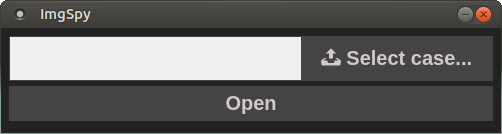
\includegraphics[width=0.7\textwidth]{./figures/img-spy-select-case.png}
		\caption{Img-spy case selector}
		\label{F:img-spy-select-case}
	\end{center}
\end{figure}

Once the case to work is picked, the main application window (Figure
\ref{F:img-spy-case-window}) is shown. This one contains tree tools needed to
proceed with the analysis. Each tool is represented with an icon.

\begin{figure}[htb]
	\begin{center}
		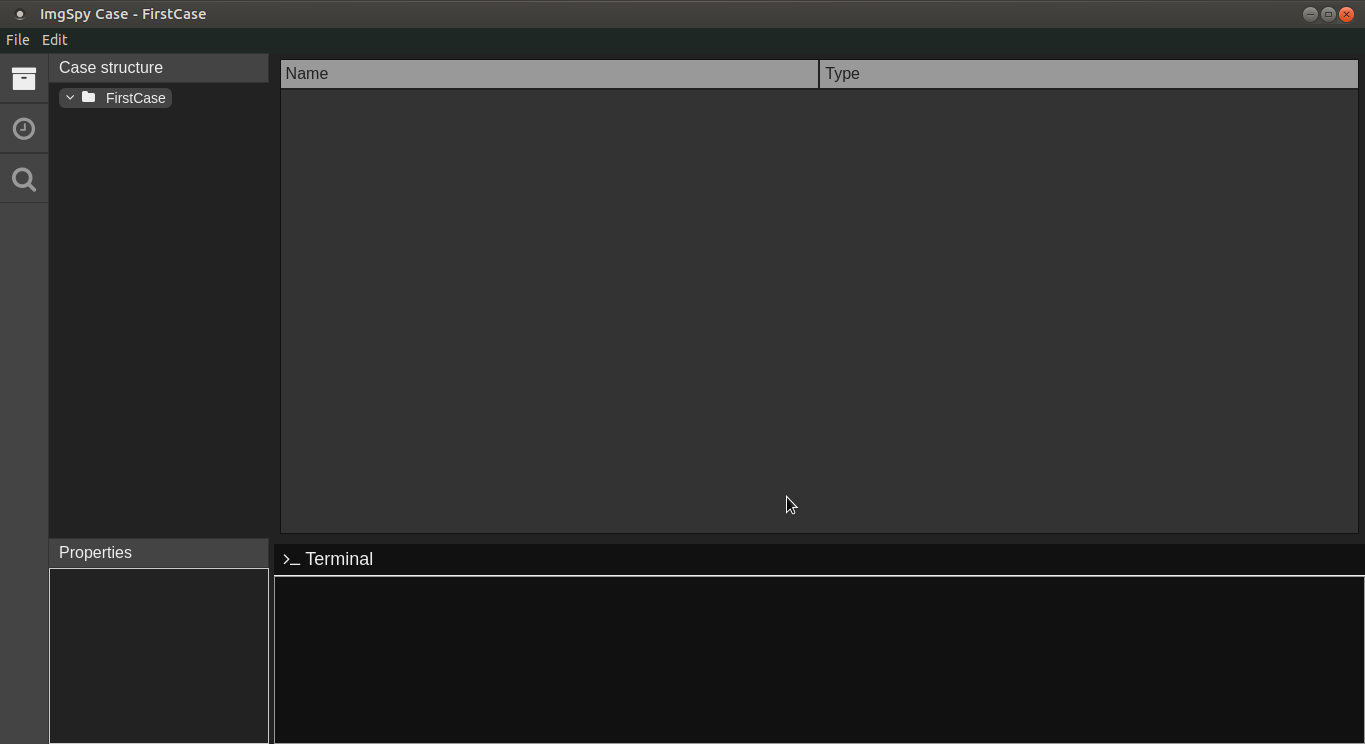
\includegraphics[width=0.7\textwidth]{./figures/img-spy-dark.png}
		\caption{Img-spy case window}
		\label{F:img-spy-case-window}
	\end{center}
\end{figure}


\begin{itemize}
	\item[] \icon{./figures/icon-dark-explorer.png}{Explorer}
	It examines images in a non-intrusive way.

	\item[] \icon{./figures/icon-dark-timeline.png}{Timeline}
	It generates a list with the activity on the file system.

	\item[] \icon{./figures/icon-dark-search.png}{Search}
	It searches a string inside an image.

\end{itemize}

One objective of the project was to be a user-friendly user interface. Many
people find inconvenient to work many hours with a bright screen while others
prefer to have more light in order to see things clearly. For that reason
multiple themes are supported. (Figure \ref{F:img-spy-multi-theme}). 

\begin{figure}[htb]
	\begin{center}
		\begin{subfigmatrix}{2}
			\subfigure[Dark theme]
			{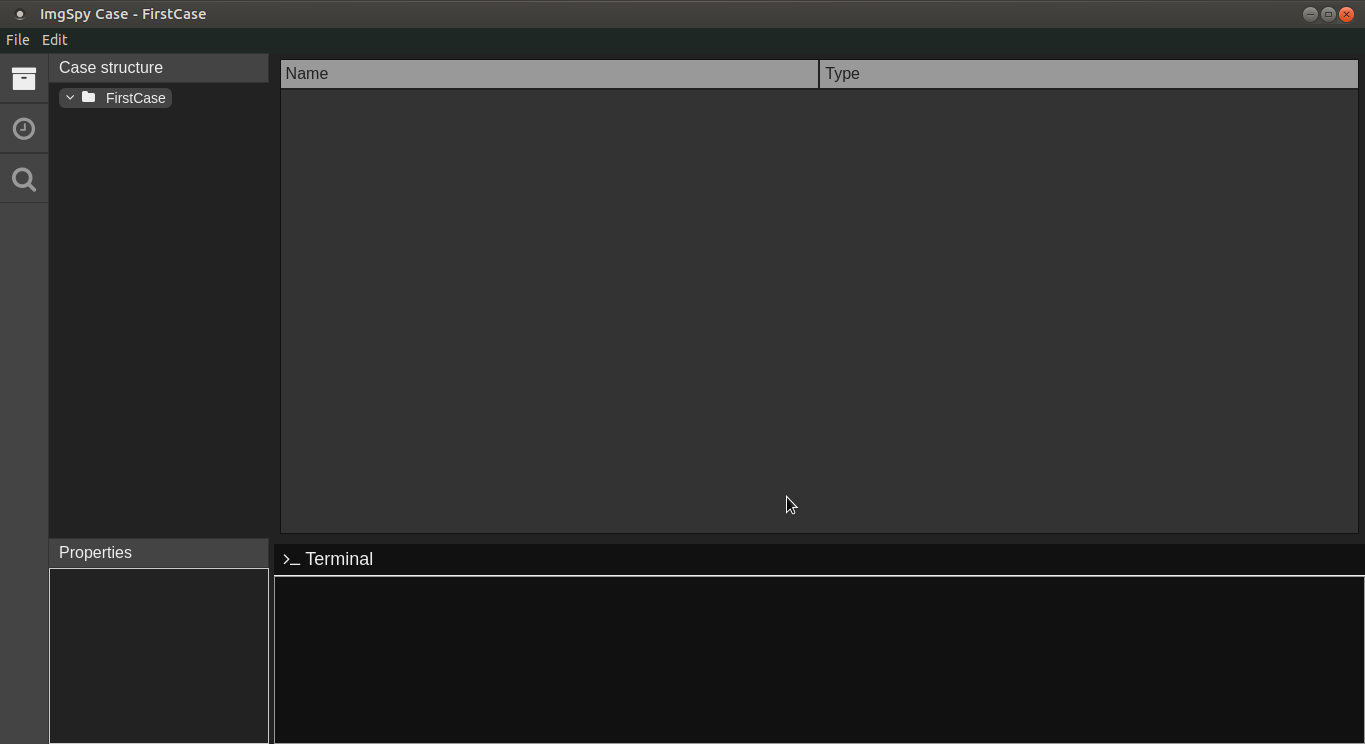
\includegraphics{./figures/img-spy-dark.png}\label{SF:S1}} 
			\subfigure[Light theme]
			{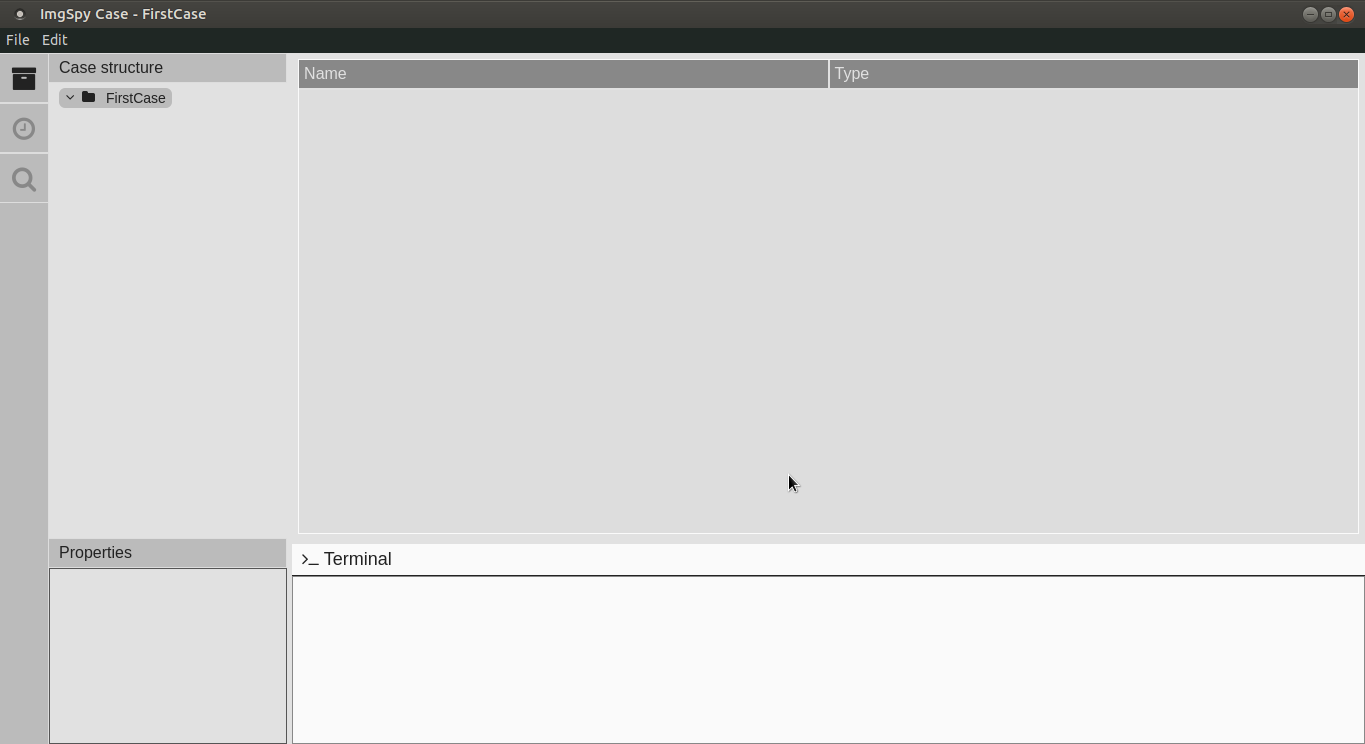
\includegraphics{./figures/img-spy-light.png}\label{SF:S1}}
		\end{subfigmatrix}
		\caption{Img-spy  multiple themes support}
		\label{F:img-spy-multi-theme}
	\end{center}
\end{figure}

\subsection{Explorer}

As seen before, \textit{Explorer} examines images in a non-intrusive way. To do
that, tsk-js analyze, list and get functions are used. Its layout contains four
panels: case structure, properties, active item content and terminal. The size
of all panels can be changed to let user feel more comfortable with the 
interface.

\subsubsection{Case structure}
\label{S:case-structure}

All folders inside the selected case folder are shown using a tree in this 
panel (Figure \ref{F:img-spy-explorer-case-structure}).

\begin{wrapfigure}[18]{L}{4.9cm}
	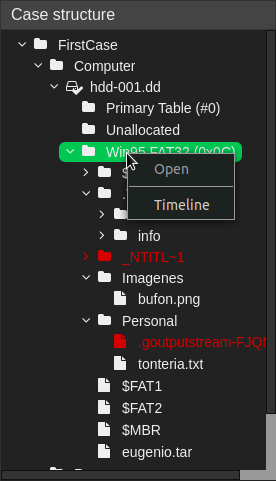
\includegraphics[width=4.4cm]{./figures/explorer-case-structure.png}
	\centering
	\caption{Explorer case structure panel}
	\label{F:img-spy-explorer-case-structure}
\end{wrapfigure}

The \textit{Explorer} is always watching case folder file system and each
change is detected launching an action to updates the application global state
refreshing the case structure tree. 

If one file have the extension \textit{.dd}, function tsk-js analysis is
executed in parallel and the image digest is computed. Once the proper hash is
provided on the image properties panel (Chapter \ref{S:explorer-properties}),
the content inside the image is added into the case tree using tsk-js list
function. Items in red color are deleted.

Each item tree have a context menu. All files can be opened with the OS
preferred applications with the open option.

Folders inside an image also have an option to generate a timeline. In case of
a disk image, partitions are treated as directories.

Finally, files have an option to export its content using tsk-js get function.

\subsubsection{Properties}
\label{S:explorer-properties}

\begin{wrapfigure}[10]{R}{6cm}
	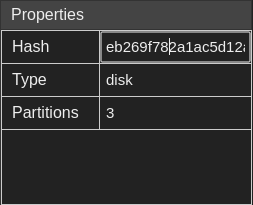
\includegraphics[width=5.5cm]{./figures/explorer-properties.png}
	\centering
	\caption{Img-spy explorer properties}
	\label{F:img-spy-explorer-properties}
\end{wrapfigure}

This panel (Figure \ref{F:img-spy-explorer-properties}) shows the properties of
the item selected on case structure (Chapter \ref{S:case-structure}).
Image properties are:

\begin{description}
	\item[Hash] This is the only editable field. Is the expected digest of the 
	image. 

	\item[Type] This value is retrieved from the tsk-js analysis. Can be disk
	or partition.
	
	\item[Partitions] If type is disk, it shows up the number of partitions
\end{description}

\subsubsection{Active item}

It displays the information of current selected item on case structure (Chapter
\ref{S:case-structure}).

\begin{figure}[htb]
	\begin{center}
		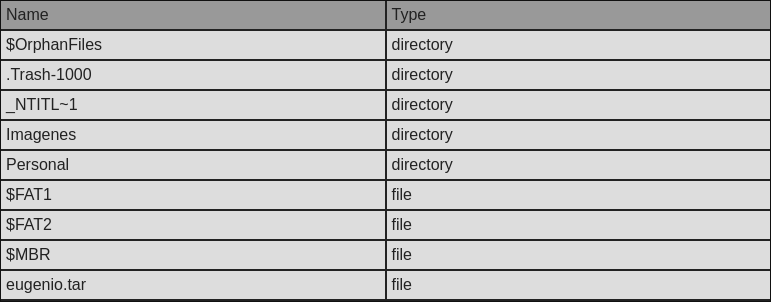
\includegraphics[width=0.7\textwidth]
		{./figures/explorer-active-folder.png}
		\caption{Img-spy active panel with a folder selected}
		\label{F:img-spy-active-folder}
	\end{center}
\end{figure}

On the one hand, when a folder is selected, active panel shows the files inside
it (Figure \ref{F:img-spy-active-folder}). If the user clicks one row, the
current active item will be the clicked one, updating also the case structure
(Chapter \ref{S:case-structure}).

\patchcmd{\subfigmatrix}{\hfill}{\hspace{0.2cm}}{}{}
\begin{figure}[htb]
	\begin{center}
		\begin{subfigmatrix}{2}
			\subfigure[Hexadecimal view]
			{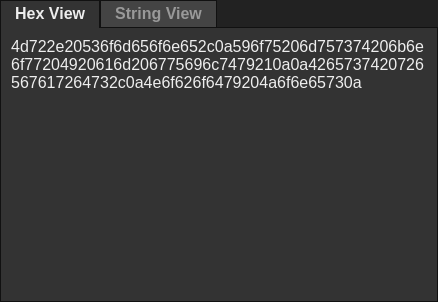
\includegraphics[width=0.4\textwidth]
			{./figures/explorer-active-file-hex.png}} 
			\subfigure[String view]
			{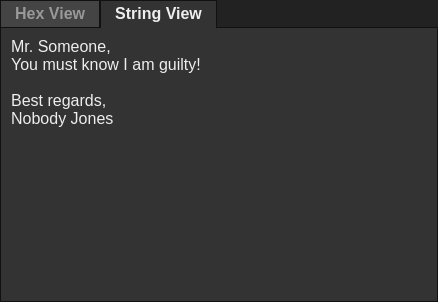
\includegraphics[width=0.4\textwidth]
			{./figures/explorer-active-file-string.png}}
		\end{subfigmatrix}
		\caption{Img-spy active panel with a file selected}
		\label{F:img-spy-active-file}
	\end{center}
\end{figure}

On the other hand, Figure \ref{F:img-spy-active-folder} shows the active panel
when a file is selected. Since the content type of the files is not known,
two type of views are supported: hexadecimal and string. It only displays
the first thousand characters to not freeze the user interface. A future line
of the project is to implement a view more functionality.

\subsubsection{Terminal}

There are many asynchronous tasks that keep some time to be executed, for 
instance, tsk-js analysis. The terminal logs those tasks and possible outputs.
Figure \ref{F:img-spy-explorer-terminal} shows some logs.


\begin{figure}[htb]
	\begin{center}
		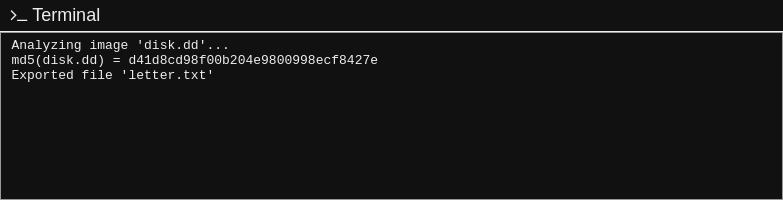
\includegraphics[width=0.9\textwidth]
		{./figures/explorer-terminal.png}
		\caption{Img-spy explorer terminal}
		\label{F:img-spy-explorer-terminal}
	\end{center}
\end{figure}

\subsection{Timeline}
\label{S:timeline}

The second tool, \textit{Timline}, generates a table with all file system
actions. Case structure context menu from \textit{Explorer} (Chapter
\ref{F:img-spy-explorer-case-structure}) has an option to generate those
tables. The function tsk-js timeline is executed to get this information.

\begin{wrapfigure}[10]{R}{5cm}
	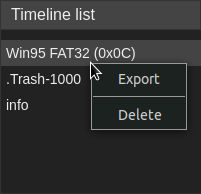
\includegraphics[width=4.5cm]
	{./figures/timeline-list.png}
	\centering
	\caption{Img-spy timeline list}
	\label{F:img-spy-timeline-list}
\end{wrapfigure}

The generation of timelines is computed on parallel using a child of electron's
main process. Some items are received with short periods of time. Instead of 
delivering one action each time an item is received, in order to reduce
unnecessary fast renderings, timeline results are buffered and delivered each
100ms at most.

\subsubsection{Timeline list}

Timeline list (Figure \ref{F:img-spy-timeline-list}) contains all generated
timelines. When its generation is finished, the data of the timeline is stored
on the current case settings and thus auto-saved.

Each item of the list has a context menu export a timeline using CSV format.
The other button is used remove the timeline item from the list and settings.

\subsubsection{Timeline table}

The timeline table (Figure \ref{F:img-spy-timeline-table}) contains the results
of a specific timeline. The user can order columns clicking the headers and 
move to different pages using previous and next buttons.

\begin{figure}[htb]
	\begin{center}
		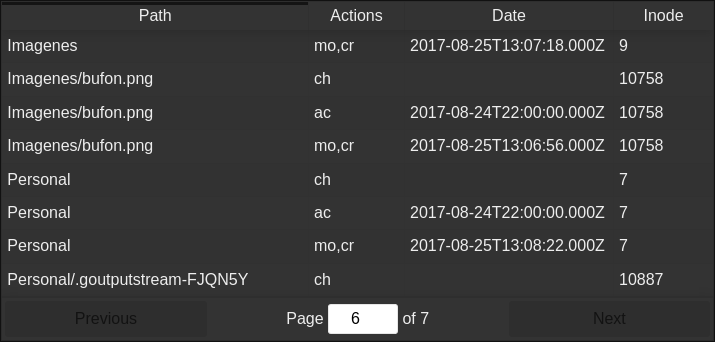
\includegraphics[width=0.8\textwidth]
		{./figures/timeline-table.png}
		\caption{Img-spy timeline table}
		\label{F:img-spy-timeline-table}
	\end{center}
\end{figure}

The fist column is the item path and the second one are the two first letters of
the actions (created, modified, changed and accessed). Then the date of the 
action, and the last is the inode.

\subsection{Search}

Finally, \textit{Search} uses tsk-js search functionality to let the
user look for a string inside the image. This execution is executed in parallel
and when all results are retrieved, they are saved on settings, as
\textit{Timeline} (see Chapter \ref{S:timeline}).

\subsubsection{Search from}

\begin{wrapfigure}[10]{L}{5.5cm}
	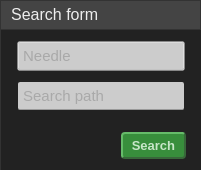
\includegraphics[width=5cm]
	{./figures/search-form.png}
	\centering
	\caption{Img-spy search form}
	\label{F:img-spy-search-form}
\end{wrapfigure}

Search form (Figure \ref{F:img-spy-search-form}) has two inputs: needle and
search path.

\begin{description}
	\item[Needle] Text that will be looked inside the image.
	\item[Search path] This field is not editable. It has the path of the
	selected item on case structure (Chapter \ref{S:case-structure}).
\end{description}

When user clicks search button, the search process starts to look for matches
on background and each time a result is retrieved, it appears on the search
result's table.

\subsubsection{Search list}

\begin{wrapfigure}[9]{R}{6cm}
	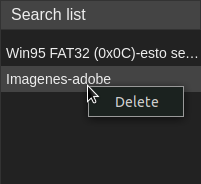
\includegraphics[width=5cm]
	{./figures/search-list.png}
	\centering
	\caption{Img-spy search list}
	\label{F:img-spy-search-list}
\end{wrapfigure}

All queried search appears on search list (Figure
\ref{F:img-spy-search-list}). When the look up finishes, it is stored on the
current case settings and thus auto-saved.

Each item of the list has a context menu with the option to delete this item
from the list and settings.

\subsubsection{Search results}

The results of the selected search item are displayed on a table inside this
panel (Figure \ref{F:img-spy-search-results}). This table, as \textit{Timeline}
table, also supports custom order by clicking the headers.

The first column shows the path of the files that contains the needle and 
how many times it appears. If the toggle button is clicked, the row
uncollapses and shows the context and index where the string if appears inside
this file.

\begin{figure}[htb]
	\begin{center}
		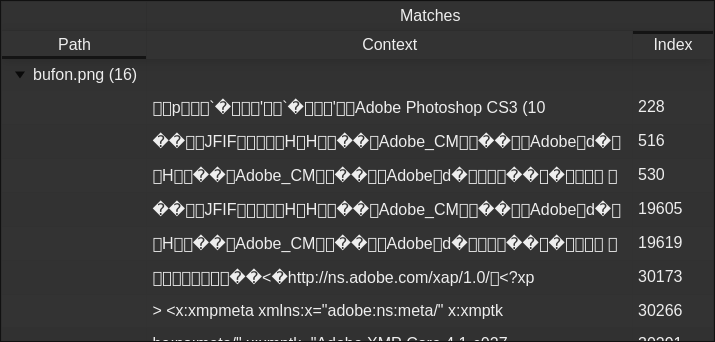
\includegraphics[width=0.8\textwidth]
		{./figures/search-results.png}
		\caption{Img-spy search results}
		\label{F:img-spy-search-results}
	\end{center}
\end{figure}

\section{Key developments}

There were many difficult or interesting parts on the development of this 
project. Some of them are multiple themes support, file system watcher, 
auto-save settings, tsk-js workers and resize panels. Also, some plug-ins where
used to increase the development speed.

\subsection{Multiple themes support}

When designing user interfaces, colors are very important. A good consideration
is to take profit of SASS define palettes and work with them. That way, to
support multiple themes is as easy select some palettes to work. The palette
format used is the one defined by Google Materials \cite{google-materials-web}.
Each theme has:

\begin{description}
	\item[Main palette] Is used for the main layout.
	\item[Primary palette] Define colors for components that must be
	highlighted.
	\item[Warn palette] Notifies the user that something is wrong. Red palette
	is normally used.
	\item[Background] Default background color.
	\item[Foreground] Default foreground color.
\end{description}


\subsection{File system watcher}

A React component has been created to launch redux actions notifying file
system changes. It uses Node.js package \textit{"chokidar"} to watch those
changes efficiently. Watcher is bound using \textit{"componentWillMount"}
lifecycle function.

Then, several Redux-Observables epics chain actions, such as, launch tsk-js
analysis function if the payload contains an image.

\subsection{Auto-save settings}

To implement the auto-save functionality, some epics actions map to update
settings model action. The auto-save epic (Listing \ref{L:auto-save-epic})
launch another to save them inside the user's disk.

\begin{codefigure}
	\tsexternal[
		classoffset=1,
		morekeywords={EpicObservable, ImgSpyState},
		%
		caption=Mapping example,
		label=L:auto-save-epic,
	]{source/auto-save.epic.ts}
\end{codefigure}

\subsection{The Sleuth Kit JavaScript workers}

As explained before, JavaScript doesn't support multithreading (Chapter
\ref{S:electron}). To do not freeze any Electron process while performing
tsk-js tasks, main process launch four subprocesses.

Those subprocesses act as workers. Each time a task is received, if any worker
is free, it takes this tasks and execute it. If none is free, the task is 
queued.

\subsection{Resize-panels}

An other React component was created to perform the resizing of panels. This
component launch a resize-start Redux action when the slider is mouse down, a
resize when the user moves the mouse and a resize-stop when the mouse is 
released.

Each time those actions are received, the resize-panel refresh its children
size using CSS properties.

\subsection{React plug-ins}

All the application forms uses \textit{react-redux-form} package. It provides
React components that store the form model inside the redux state. In this
manner, the form values are accessible from any other React component.

Timeline and Search result tables are drawn using \textit{react-tables}. This 
package has React components to render tables very fast. Those tables have 
order by, pagination and row aggregation functionalities implemented.

\section{Code quality analysis}

% TODO: No se si es interesante poner esto aunque creo que da una idea de como
% esta hecho

To check if the project is scalable enough, some code quality metrics are 
calculated. The command used is \textit{sloc}.


\begin{terminal}[
	caption=Code quality CSV extraction using sloc,
	label=L:sloc-code-quality
]
%
\terminalcmd[sloc -d -f csv -e lib src/ > code-quality.csv]
%
%\terminalcmd%

\end{terminal}

With this information, some interesting metrics can be computed. Table

\begin{table}[htb]
\begin{center}
\begin{tabular}{|l|l|l|}
\hline
{\bf Metric }	& {\bf Value} & {\bf Expected} \\ \hline \hline
Total files & 190 & - \\ \hline
Source lines & 8779 & - \\ \hline
\hline

Max. source lines per file & 301 & \textless\space\text{300} \\ \hline
Min. source lines per file & 1 & \textgreater\space\text{1} \\ \hline
Avg. source lines per file & \approxtext\text{46} & \textless\space\text{100} \\ \hline
\hline
Files without comments & 70.5\% & \textless\space\text{20\%} \\ \hline
Comments / Source & 2\% & \textgreater\space\text{5\%} \\ \hline
Avg. code blocks size & 4 & - \\ \hline
\end{tabular}
\caption{Code analysis metrics}
\label{T:code-analysis-metrics}
\end{center}
\end{table}







\cleardoublepage
\phantomsection
\chapter*{Conclusions}

The development of a cross-platform digital forensics applications is a long
process with many key decisions. The first one is to choose a technological
environment. This task is not that easy due to the great amount of
very-different solutions. But, nowadays web technologies are standing strong in
terms of cross-platform compatibility. \textbf{A well-known solution} that many
companies are using today is \textbf{Electron} \cite{electron-web}, which uses
Chromium as library to instantiate Chrome windows. 

Once the work environment is well-defined, an overview of the application 
should be provided. The software architecture defines it by using black boxes
and defining their interactions. Model-view-controller (MVC) is a mature
widely-used architecture. Its main disadvantage is that becomes complex when
increasing the number of views with interaction between themselves. Since
this is the case of the application we have developed, MVC is not a good
architecture in this case.

The direct evolution of MVC is Flux, which was defined by Facebook to fix its
scalabilty problem. In order to solve this problem, Flux purposes the use of
a unique state to render whole the application. In this project we have
used \textbf{React-Redux} to build  \textbf{flux-like architecture}
Nevertheless, other libraries, such as Redux-Observables, have been used in
order to address React-Redux lacks.

With those good bases, a complete application can be build but there is still a
need to implement the computationally complex operations of the digital 
forensics work flow. Those have to be coded in a low programming language to
guarantee a good efficiency. The Sleuth Kit provides a C library that
implements those operations. Therefore, \textbf{The Sleuth Kit JavaScript, a
Node.js wrapper, has been created} to let JavaScript use those operations.

Finally, \textbf{Img-Spy, the digital forensics application developed to fulfill
the goal of this project, defines three tools}: \textit{Explorer},
\textit{Timeline} and \textit{Search}. Those tools let an investigator to
analyze the file system of an image in a non-intrusive way, create a timeline
based on actions performed on the disk and search which files contain a
specific string.

During the development process, many interesting or difficult tasks where found,
for instance, watching changes on the file system of user's computer, performing
actions in parallel using JavaScript and defining a user-friendly interface
supporting, for example, resize-panels or multiple themes.

Looking ahead, many optimizations and features can be added to Img-spy. First,
\textit{Explorer} tool can be improved in terms of performance adding Redux
selectors and reducing React rerenders. Also, the hash is always computed
without asking the user, consuming too many resources that are not always
required.

\textit{Timeline} tool can be also improved by adding graphs to represent those
actions in a more visual way. Add filters can also help investigators to remove
useless information. For instance, a useful filter could be to see just the
files of a specific search result.

In many cases, search files by name is also needed. Therefore, \textit{Search}
tool can implement this operation. More custom searches can be executed using
Regex.

There is a saying that “Programming can be fun, so can cryptography; however
they should not be combined” \cite{code-complete}. So regarding code quality,
comments can be added to help new developers understand easily how the software 
works.

Finally, new tools can be added in order to detect mismatches on file 
extensions or to help investigators to write the final report. Just take always
into account that, as Gordon Bell said:

\begin{quote}
	“Every big computing disaster has come from taking too many ideas and putting them in one place”.
\end{quote}

%%%  BIBLIOGRAFIA
%%%%%%%%%%%%%%%%%%%%%%%%%%%%%%%%%%%%%%%%%%%%%%%%%%%%%%%%%%%%%%%%%%%%%%%%%%

%%% Per la bibliografia hi ha 2 opcions: generarla amb la utilitat BibTeX 
%%%                                      o fer-la ''a ma''
%%% NOTA: podeu trobar facilment informació sobre BibTeX a:
%%%  http://www.ctan.org/tex-archive/biblio/bibtex/contrib/doc/

%%% OPCIO 1: BibTeX (recomanat) -> descomentar les comandes seguents:
% \bibliographystyle{apacite}
\bibliographystyle{unsrt}   %% Estil de bibliografia EETAC 
\cleardoublepage \phantomsection % Indicar aqui el(s) fitxer(s) que contenen la bibliografia
\bibliography{plantilla_tfc}
% \pdfbookmark{<Bibliography}{sec:biblio}
%%% OPCIO 2: bibliografia manual
%%%
%%% L'argument d'entrada es el numero de referencies que s'inclouen
%\cleardoublepage \phantomsection \begin{thebibliography}{2}

%% Llibres:  Autor/s (cognoms i inicials dels noms), títol del llibre (en 
% cursiva), editor, ciutat i any de publicació. Quan es cita el capítol d'un
% llibre s'ha d'indicar el títol del capítol (entre cometes), el títol del
% llibre (en cursiva) i els números de pàgines amb la primera i la darrera
% incloses.

%%  Exemple de capitol en llibre
%\bibitem{prova1} Cognoms-autor, Inicial-nom.  ``Títol del capítol''. {\it Títol
%	del llibre}.  (Editor. Ciutat. Any publicació): pagina1--paginaN.

%%  Exemple de d'article en revista
%\bibitem{prova2} Cognoms-autor, Inicial-nom.  ``Títol de l'article''. {\it
%	Títol de la revista}.  {\bf volum}(numero), pagina1--paginaN. (Any
%		publicació) 

%\end{thebibliography}



%%%%%%%%%%%%%%%%%%%%%%%%%%%%%%%%%%%%%%%%%%%%%%%%%%%%%%%%%%%%%%%%%%%%%%%%%%
%%%%%%                           APENDIXS                         %%%%%%%%
%%%%%%%%%%%%%%%%%%%%%%%%%%%%%%%%%%%%%%%%%%%%%%%%%%%%%%%%%%%%%%%%%%%%%%%%%%
\pagestyle{empty}  % no tocar

%% Descomentar una de les dues línies següents, en funció de:
%%  a) els apendixs s'encuadernaran apart (amb portada) 
%%  b) els apendixs s'enquadernen amb el mateix projecte (sense portada). 
%% Recordeu que si tot el document (amb apèndixs) excedeix les 100 pagines 
%% s'ha d'enquadernar a part
%\appendix\ambportada
\appendix\senseportada


%%%%%%%%%%%%%%%%%%%%%%%%%%%%%%%%%%%%%%%%%%%%%%%%%%%%%%%%%%%%%%%%%%%%%%%%%%
%%%%%% INCLOURE A PARTIR D'AQUI TOTS ELS CAPÍTOLS DELS APENDIXS   %%%%%%%%
%%%%%%%%%%%%%%%%%%%%%%%%%%%%%%%%%%%%%%%%%%%%%%%%%%%%%%%%%%%%%%%%%%%%%%%%%%

\chapter{Electron hello world}
\label{APP:electron-hello-world}

This example is based on the
\href{https://github.com/electron/electron-quick-start/}{electron quick start}.

\begin{codefigure}
	\htmlexternal[
		caption=Electron index HTML file,
		label=L:electron-index-html
	]{source/electron-hello-world.html}
\end{codefigure}

\begin{codefigure}
	\jsexternal[
		caption=Electron menu creation,
		label=L:electron-menu,
		%
		classoffset=1,
		morekeywords={BrowserWindow}
	]{source/electron-menu.js}
\end{codefigure}

\begin{codefigure}
	\jsexternal[
		caption=Electron main,
		label=L:electron-main,
		%
		classoffset=1,
		morekeywords={BrowserWindow}
	]{source/electron-hello-world.js}
\end{codefigure}

\chapter{The Sleuth Kit JavaScript typings}
\label{APP:tsk-js-typings}

A typings file is a TypeScript file that only contains types. It is used by
TpyeScript to detect type mismatches.

\begin{codefigure}
	\tsexternal[
		caption=The Sleuth Kit JavaScript typings,
		label=L:tsk-js-typings,
		%
		classoffset=1,
		morekeywords={
			TSK, ImgInfo, TskOptions, ImgFile, TimelineCallback,
			TimelineItem, SearchCallback, PartitionInfo, DiskAction
		},
	]{source/tsk-js-typings.ts}
\end{codefigure}

% \chapter{Definitions}

\begin{description}
	\item [Open source software]
	Very well Manuel

	\item [Cross-platform software]
	Very well Fandango

	\item [Operative System (OS)]
	Very well Manuel

	\item [Library (programming)]
	Very well 

	\item [Hello World program]
	Very well World

\end{description}



%%%%%%%%%%%%%%%%%%%%%%%%%%%%%%%%%%%%%%%%%%%%%%%%%%%%%%%%%%%%%%%%%%%%%%%%%%
%%%%%%%%%%%%%%%%%%%%%%%%%%%%%%%%%%%%%%%%%%%%%%%%%%%%%%%%%%%%%%%%%%%%%%%%%%
%%%%%%%%%%%%%%%%%%%%%%%%%%%%%%%%%%%%%%%%%%%%%%%%%%%%%%%%%%%%%%%%%%%%%%%%%%
% i  aixo es tot! ;)
\end{document}






